% Bayesian Uncertainty Calibration & OOD Detection for Oncological Scans
%
% Compiling:
%   * On Overleaf, start from the official NeurIPS 2024 template and drop this
%     file in; it will pick up neurips_2024.sty automatically.
%   * Standalone (no .sty available), the fallback preamble below reproduces the
%     NeurIPS page geometry closely enough to read and to page-count.
%
% Numbers come from paper/tables.tex and paper/macros.tex, both generated by
% paper/make_tables.py from results/*.json. Do not hand-edit them.

\documentclass{article}

\IfFileExists{neurips_2024.sty}{%
  \usepackage[final]{neurips_2024}%
}{%
  % --- fallback: approximate the NeurIPS layout ------------------------
  % neurips_2024.sty loads natbib itself; the fallback must, or every \citep
  % becomes an undefined control sequence and the citations silently vanish
  % from the PDF while the build still "succeeds".
  \usepackage[letterpaper, margin=1.5in, top=1.0in, bottom=1.0in]{geometry}
  \usepackage{times}
  \usepackage[round]{natbib}
  \renewcommand{\baselinestretch}{0.99}
  \setlength{\parskip}{0pt}
}

\usepackage[utf8]{inputenc}
\usepackage[T1]{fontenc}
\usepackage{hyperref}
\usepackage{url}
\usepackage{booktabs}
\usepackage{amsfonts}
\usepackage{amsmath}
\usepackage{amssymb}
\usepackage{microtype}
\usepackage{graphicx}
\usepackage{subcaption}

\hypersetup{colorlinks=true, linkcolor=black, citecolor=black, urlcolor=blue}

\DeclareMathOperator*{\E}{\mathbb{E}}
\DeclareMathOperator{\Var}{Var}
\newcommand{\Hent}{\mathbb{H}}
\newcommand{\MI}{\mathbb{I}}

% figures/full first: the paper reports the full study. figures/quick is a
% fallback so the document is still readable while a run is in progress -- but
% build.sh greps the log and warns loudly if any figure was resolved from there,
% because a full-study paper illustrated with smoke-test plots is a lie that
% compiles cleanly.
\graphicspath{{../figures/full/}{../figures/quick/}{../figures/}{figures/}}
% GENERATED by paper/make_tables.py -- do not edit by hand.
\newcommand{\bracketLo}{0.514}
\newcommand{\bracketHi}{0.547}
\newcommand{\bracketWidth}{0.034}
\newcommand{\zCorr}{0.844}
\newcommand{\fittedT}{1.00}
\newcommand{\eceRaw}{0.017}
\newcommand{\eceCal}{0.019}
\newcommand{\nllRaw}{0.530}
\newcommand{\nllCal}{0.531}
\newcommand{\testAcc}{0.733}
\newcommand{\novelAcc}{0.728}
\newcommand{\decoupledAcc}{0.507}


\title{Validating Uncertainty Decomposition Against a Known Posterior:\\
A Phantom Benchmark for Oncological Screening}

\author{%
  Ibrahim Laklaa \\
  \texttt{https://github.com/X1-Il/bayesian-uncertainty-oncology}
}

\begin{document}
\maketitle

\begin{abstract}
Uncertainty estimates for medical imaging are almost always evaluated by proxy.
On real scans there is no ground truth for how ambiguous an image is, so a
reported ``aleatoric entropy'' can be checked only through downstream surrogates
--- calibration error, OOD ranking, deferral curves --- none of which can say
whether the estimate is \emph{numerically correct}. We take the opposite route
and study uncertainty on a synthetic screening benchmark whose generative process
is written down, so the Bayes-optimal posterior, the Bayes error, and the
irreducible label entropy are all available in closed form. This converts the
usual benchmark run into a falsifiable experiment: each term of the standard
epistemic/aleatoric decomposition acquires a target value.
%
The oracle is not assumed valid. It holds only if the latent biomarker is
recoverable from the image, which is false in the tails, so we \emph{bracket} it:
the analytic value is a lower bound on attainable aleatoric entropy, and a
deliberately suboptimal matched-filter estimator supplies an upper bound
$[\bracketLo, \bracketHi]$ nats. A correct estimate must land inside.
%
We then evaluate what the decomposition buys downstream --- calibration under ten
distribution shifts, six OOD scores, and selective prediction on a mixed stream.
Four negative results are reported as prominently as the positive ones, because
each corrects a claim we initially expected to make. The sharpest: on a condition
where the image remains in distribution but carries no information about the
label, the model sits at chance accuracy with three times the calibration error
of any other split, and \emph{every} out-of-distribution score --- softmax,
entropy, energy, epistemic mutual information, Mahalanobis --- is at chance.
Since each is a function of $x$ and the corruption lies in $p(y \mid x)$ rather
than $p(x)$, this is an impossibility rather than a tuning failure, and it bounds
what OOD detection can contribute to clinical safety. Temperature scaling is a
\emph{null} on this model ($T \approx 1$, no ECE improvement): a deep ensemble
with a heteroscedastic head is already calibrated, so we add a deliberately
miscalibrated baseline to distinguish ``the correction does not work'' from ``the
model did not need it''. An unseen lesion \emph{morphology} turns out not to be a
semantic shift at all, because the rendering still encodes the latent in its
contrast --- accuracy is unchanged --- so we construct a \texttt{decoupled}
condition that severs the image--label link instead. And the argmax-invariance
guarantee of temperature scaling, routinely quoted for ensembles, does not
survive the mixture: we measure the accuracy shift rather than assume it away.
Code, tests of the mathematical identities, and all figures are released.
\end{abstract}

\section{Introduction}

In cancer screening a model that is wrong is survivable; a model that is wrong
\emph{and confident} is not. This motivates treating the predictive distribution,
rather than the prediction, as the object of study. The standard toolkit is
mature: predictive uncertainty decomposes exactly into an epistemic and an
aleatoric part \citep{houlsby2011bald, depeweg2018decomposition}, approximate
posteriors are available through MC dropout \citep{gal2016dropout} and deep
ensembles \citep{lakshminarayanan2017ensembles}, input-dependent label noise can
be learned \citep{kendall2017uncertainties}, and probabilities can be corrected
post hoc \citep{guo2017calibration}.

What is missing is validation. Every component above is evaluated on datasets
where the quantity being estimated is unobservable. If a model reports
$0.31$ nats of aleatoric uncertainty on a mammogram, nothing in the dataset can
confirm or refute it. The field therefore evaluates uncertainty through proxies
that are individually reasonable and jointly incapable of detecting a
systematically wrong estimate --- a miscalibrated-but-well-ranked estimator
scores well on AUROC, and a well-calibrated-but-uninformative one scores well on
ECE.

\paragraph{Contributions.}
\begin{enumerate}\itemsep2pt
\item A screening benchmark whose posterior $p^*(y \mid x)$, Bayes error and
irreducible entropy are known in closed form, with a tunable dial $\beta$
controlling how much label noise exists (Section~\ref{sec:benchmark}).
\item An \emph{identifiability bracket} rather than an assumed oracle: we bound
the attainable aleatoric entropy from both sides and require estimates to land
inside, which makes the benchmark's central claim checkable
(Section~\ref{sec:bracket}).
\item Two falsification experiments no real dataset supports --- recovery of the
analytic label noise across a $\beta$ sweep, and the decay of the epistemic term
with data at fixed aleatoric (Sections~\ref{sec:e1}--\ref{sec:e2}).
\item A \texttt{decoupled} shift condition that isolates semantic novelty from
novelty of appearance, together with the measurement showing why the obvious
alternative --- an unseen lesion morphology --- does not (Section~\ref{sec:benchmark}).
\item A downstream evaluation carrying the aleatoric term as an explicit negative
control for OOD detection, and three corrections to claims the standard toolkit
invites: that post-hoc calibration is generally needed, that unfamiliar
appearance implies unfamiliar task, and that temperature scaling preserves the
accuracy of an ensemble (Sections~\ref{sec:e3}--\ref{sec:e6}).
\end{enumerate}

\paragraph{Reproducibility.} Every number in this report is generated directly
from the released result files; none is transcribed by hand. The mathematical
identities the analysis relies on --- the decomposition
\eqref{eq:decomp}, the law of total variance, argmax invariance, rank-based
AUROC with ties, and the invariance of AURC under monotone reparameterisation ---
are enforced by unit tests rather than asserted in prose.

\section{Background}

Let $q(w)$ be an approximate posterior over weights, giving the predictive
distribution $p(y \mid x) = \E_{q(w)}[p(y \mid x, w)]$. The decomposition
identity is
\begin{equation}
\underbrace{\Hent\!\left[\E_{q(w)} p(y \mid x, w)\right]}_{\text{total}}
= \underbrace{\MI(y ; w \mid x)}_{\text{epistemic}}
+ \underbrace{\E_{q(w)} \Hent\!\left[p(y \mid x, w)\right]}_{\text{aleatoric}} .
\label{eq:decomp}
\end{equation}
Total uncertainty splits into the part that disagreement between plausible models
explains, and the part every plausible model agrees is irreducible. Both terms
are non-negative, so \eqref{eq:decomp} is a genuine decomposition rather than a
heuristic split, and the epistemic term is exactly the mutual information between
the label and the weights --- zero if and only if every posterior sample predicts
identically.

Two consequences make \eqref{eq:decomp} testable, and they are the basis of our
experiments: the epistemic term must vanish as the training set grows, while the
aleatoric term must converge to a constant fixed by the data-generating process
and \emph{not} respond to more data.

A second route via the law of total variance,
$\Var[p] = \E_q[\Var(p \mid w)] + \Var_q[\E(p \mid w)]$, decomposes the same way
through a different functional; we compute it alongside as a cross-check.

\section{A phantom benchmark with a known posterior}
\label{sec:benchmark}

\paragraph{Generative model.}
For each scan we draw a scalar latent biomarker $z \sim \mathcal{N}(0,1)$ and
sample the label from a logistic link,
\begin{equation}
p^*(y = 1 \mid z) = \sigma(\beta z), \qquad \sigma(t) = (1 + e^{-t})^{-1}.
\label{eq:link}
\end{equation}
The image is rendered as $x = \mathrm{render}(z, \nu)$, where the nuisance
variables $\nu$ --- head shape and orientation, lesion position and radius, tissue
texture, bias field, pixel noise --- are independent of $y$ given $z$. The latent
is encoded as \emph{signed} lesion contrast, so $z>0$ renders a hyper-intense
lesion and $z<0$ a hypo-intense one.

Because $\nu \perp y \mid z$, the chain $y - z - x$ gives
$p^*(y \mid x) = p^*(y \mid z(x)) = \sigma(\beta z)$, \emph{provided} $z$ is
recoverable from $x$. The dial $\beta$ controls irreducible noise: as
$\beta \to \infty$ the problem becomes separable, as $\beta \to 0$ it becomes a
coin flip. The Bayes error $\E_z[\min(p^*, 1-p^*)]$ and the irreducible entropy
$\E_z[\Hent(p^*)]$ follow in closed form.

\begin{figure}[t]
\centering
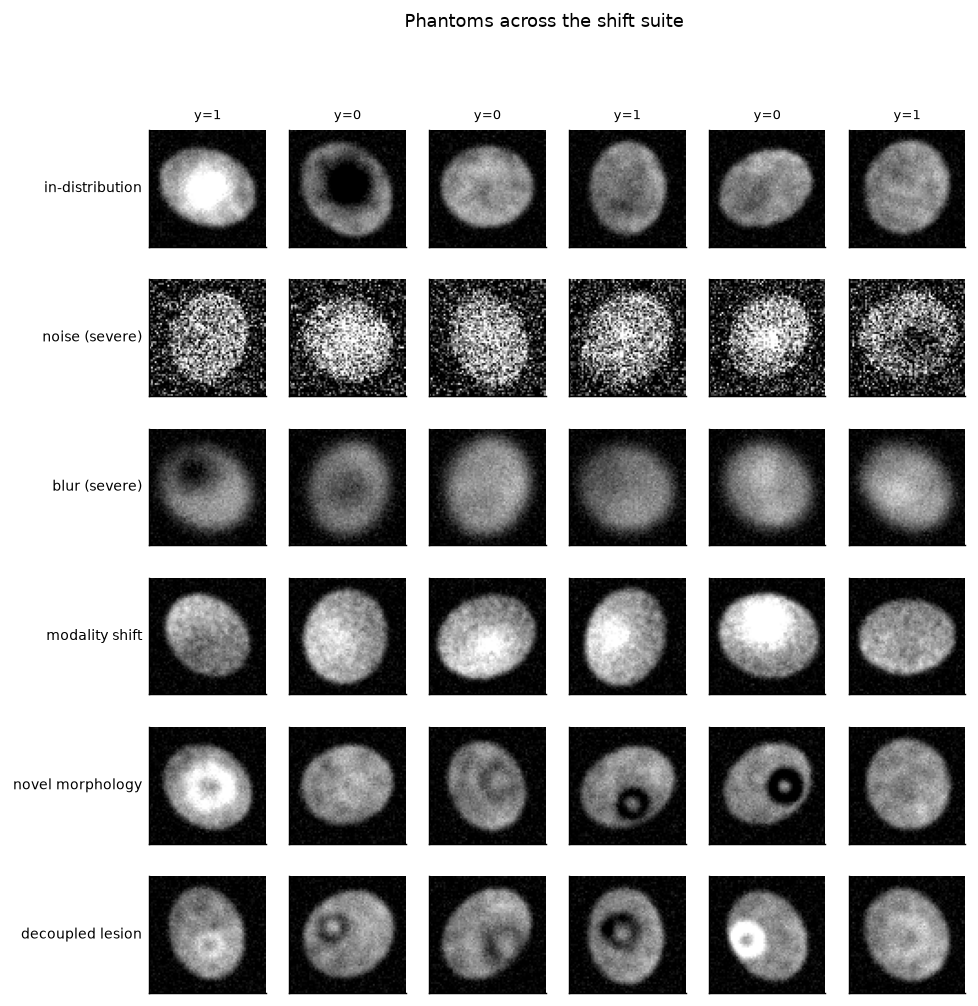
\includegraphics[width=\linewidth]{01_phantoms.png}
\caption{\textbf{The benchmark.} Rows: in-distribution, severe noise, severe blur,
modality shift, and novel (annular) morphology. The latent $z$ is encoded as
\emph{signed} lesion contrast, so ambiguity is a smooth function of conspicuity
rather than a discrete label-flip, and the label above each column is a
\emph{sample} from $\sigma(\beta z)$ --- two visually identical scans can carry
opposite labels, which is precisely the irreducible noise the aleatoric term must
recover.}
\label{fig:phantoms}
\end{figure}

\paragraph{Shift suite.} Ten test conditions: Gaussian noise and blur at three
severities each, a \emph{modality shift} with inverted tissue contrast, finer
texture and a stronger bias field, an unseen \emph{annular lesion morphology},
and a \emph{decoupled} condition described below. We keep covariate and semantic
shift separate throughout, because the correct behaviour differs: stay calibrated
under covariate shift, abstain under semantic shift. Averaging them into a single
``OOD AUROC'' hides the only interesting comparison.

\paragraph{What counts as a semantic shift.} Our first attempt at semantic
novelty was the annular morphology, on the reasoning that a lesion shape absent
from training is unfamiliar. Measured, it is not: accuracy on that split is
$\novelAcc$ against $\testAcc$ in distribution, a difference inside noise, while
the corrected \texttt{decoupled} condition drops to $\decoupledAcc$ --- chance,
as its construction requires. The reason is
that the renderer still sets the lesion amplitude to $\mathrm{lesion\_amp}\cdot z$,
so the signed contrast continues to carry the latent and the network reads it off
a ring about as well as off a blob. An unseen \emph{appearance} is not an unseen
\emph{task}; this is a covariate shift wearing a semantic costume, and reporting
it as semantic would have made Section~\ref{sec:e4}'s central comparison
vacuous.

The \texttt{decoupled} condition is the corrected version: the same unseen
morphology, but with the amplitude drawn from an independent standard normal.
The image then carries no information about the label, $p^*(y\mid x) = 1/2$
exactly, and no model can beat chance --- so abstention is the only correct
response. Because the marginal appearance statistics still match training, this
isolates the severed image--label \emph{link} from any change in appearance,
which is precisely the variable E4 needs to manipulate.

\subsection{Bracketing the oracle rather than assuming it}
\label{sec:bracket}

The proviso in \eqref{eq:link} is not free. Lesion position and radius are
unknown, texture is a nuisance field, and intensity clipping at $1.0$ compresses
the tails, so $z$ is \emph{not} exactly recoverable and $p^*(y\mid x) = \sigma(\beta z)$
is not exactly the posterior. Rather than assert the oracle, we bound it.

Let $A^\star = \E_z[\Hent(\sigma(\beta z))]$ be the analytic value, and let
$\hat{A}$ be the same functional computed from a matched-filter estimate
$\hat{z}$ of the latent. Because a suboptimal estimator discards information, it
can only inflate apparent noise, so
\begin{equation}
A^\star \;\le\; A_{\text{attainable}} \;\le\; \hat{A},
\end{equation}
where $A_{\text{attainable}}$ is what a Bayes-optimal estimator of $z$ from $x$
would see. The matched filter is a fixed linear template bank while the network
may learn a better statistic, so $\hat{A}$ is a genuine upper bound. Empirically
$\mathrm{corr}(\hat z, z) = \zCorr$ and the bracket is
$[\bracketLo, \bracketHi]$ nats, a width of $\bracketWidth$. An aleatoric
estimate inside this interval is consistent with a correct estimator; one outside
is not. This is the difference between a claim that can be checked and one that
merely sounds rigorous.

\section{Method}

\paragraph{Posterior approximation.} We use both MC dropout --- channel-wise
\texttt{Dropout2d}, since element-wise masking is largely averaged away by
spatial pooling --- and a deep ensemble of independently initialised networks.
Batch normalisation is held in evaluation mode during MC sampling; letting it use
batch statistics injects a batch-composition-dependent variance that would appear
in the epistemic term and has nothing to do with weight uncertainty.

\paragraph{Aleatoric head.} Following \citet{kendall2017uncertainties} the network
emits a mean logit vector $f(x)$ and a log-variance $s(x)$, and the softmax is
integrated over logit noise: $u_t = f(x) + \sigma(x)\epsilon_t$,
$L = -\log \frac{1}{S}\sum_t \mathrm{softmax}(u_t)_y$, evaluated in log-space.
Note $\sigma(x)$ is learned without supervision: inflating it on an ambiguous
input raises the log-mean-exp of the correct-class log-probability even as it
lowers the mean logit.

\paragraph{Nested Monte Carlo.} The two sources are kept separate: $T$ weight
samples, each marginalising $S$ logit samples, giving $p(y\mid x, w_t)$ before
\eqref{eq:decomp} is applied. Drawing a single joint sample of (mask, logit
noise) and treating the spread as epistemic folds aleatoric noise into the
epistemic term --- a silent error, since the resulting numbers remain plausible.

\paragraph{Calibration.} We report ECE with equal-width and equal-mass bins, MCE,
class-wise ECE, and Murphy's decomposition
$\mathrm{BS} = \text{reliability} - \text{resolution} + \text{uncertainty}$
\citep{murphy1973}. Binned ECE is biased downward and bin-scheme dependent, and
equal-width bins under-resolve exactly the high-confidence region where
clinically relevant errors live; every ECE is therefore reported with a $95\%$
bootstrap confidence interval and compared on intervals, not point estimates.
Temperature scaling \citep{guo2017calibration} is the default correction because
its guarantee is provable: dividing every logit by the same $T>0$ is strictly
monotone, so $\arg\max$ --- and therefore accuracy --- is exactly preserved.

That theorem concerns a \emph{single} softmax, and it is routinely over-applied.
A posterior predictive is a mixture, $p = \frac{1}{M}\sum_m \mathrm{softmax}(z_m)$,
and since softmax is non-linear, mean-of-softmax $\neq$ softmax-of-mean: scaling
the \emph{averaged} logit calibrates a different estimator from the one being
reported. We therefore scale inside the average,
$p_T = \frac{1}{M}\sum_m \mathrm{softmax}(z_m/T)$, and note that for this mixture
\textbf{the argmax guarantee does not survive} --- raising $T$ flattens each
member toward uniform, which re-weights the members' contributions and can change
the winning class. Accordingly we \emph{measure} the induced accuracy shift
rather than assume it away, while still verifying the exact theorem on the
single-model object to which it applies. During development an assertion
demanding exact invariance of the mixture aborted an otherwise correct run, which
is precisely the confusion this paragraph is meant to prevent.

\paragraph{Selective prediction.} For $g(x) = \mathbf{1}[\kappa(x) \ge \tau]$,
selective risk is $R(\tau) = \E[\ell \cdot g]/\E[g]$
\citep{elyaniv2010, geifman2017selective}. Since AURC is bounded below by the
model's own error rate we report excess AURC against the oracle ranking. A
consequence worth stating: temperature scaling is monotone and therefore
\emph{cannot} change the ranking, the risk--coverage curve, or AURC. A reported
AURC improvement from temperature scaling is necessarily a bug. What calibration
buys is threshold semantics --- hitting a target risk requires the probabilities
to mean what they say.

\paragraph{OOD scores.} MSP \citep{hendrycks2017baseline}, predictive entropy,
energy $-\log\sum_c e^{z_c}$ \citep{liu2020energy}, the epistemic term
$\MI(y;w\mid x)$, and Mahalanobis distance in penultimate feature space with tied,
shrunk covariance \citep{lee2018mahalanobis}. AUROC is computed via the
Mann--Whitney identity with tie correction, which matters because several scores
saturate and a naive threshold sweep rewards that saturation. The aleatoric term
is carried as a \emph{negative control}: if it detects semantic novelty as well
as the epistemic term does, the decomposition is not separating two different
things and every other result is suspect.

\section{Experiments}

% GENERATED by paper/make_tables.py -- do not edit by hand.

\begin{table}[t]
\caption{\textbf{E1: recovery of the analytic label noise.} The target column is
$\mathbb{E}_z[H(p^*)]$, computed in closed form from the generative model, not
estimated. The aleatoric estimate tracks it across the sweep while the epistemic
term stays flat at $O(10^{-4})$ --- both from the same forward passes, so no
rescaling of ``uncertainty'' could make one column follow a moving target while
the other does not. $\Delta$ is positive at \emph{every} point, which the
identifiability argument of Section~\ref{sec:bracket} predicts in advance: a
suboptimal view of the latent can only inflate apparent noise, never deflate it.
The final column is the per-example correlation between the estimated aleatoric
term and the oracle entropy $H(p^*(y|x))$ on the same image, which an estimator
that merely matched the sweep means could not achieve.}
\label{tab:e1}
\centering
\small
\begin{tabular}{cccccccc}
\toprule
$\beta$ & target $\mathbb{E}_z[H(p^*)]$ & est.\ aleatoric & $\Delta$ &
epist.\ ($\times 10^{-3}$) & Bayes err. & model err. & corr.\ (per-ex.) \\
\midrule
0.6 & 0.653 & 0.662 & $0.0087$ & 0.29 & 0.387 & 0.396 & 0.742 \\
1.0 & 0.599 & 0.609 & $0.0102$ & 0.36 & 0.325 & 0.342 & 0.809 \\
1.6 & 0.513 & 0.540 & $0.0269$ & 0.51 & 0.256 & 0.268 & 0.863 \\
2.5 & 0.406 & 0.424 & $0.0181$ & 0.60 & 0.189 & 0.202 & 0.902 \\
4.0 & 0.290 & 0.307 & $0.0167$ & 0.56 & 0.128 & 0.144 & 0.928 \\
\bottomrule
\end{tabular}
\end{table}

\begin{table}[t]
\caption{\textbf{E2: epistemic uncertainty decays with data; aleatoric does not.}
Both columns are computed from the same forward passes, so no monotone rescaling
of ``uncertainty'' could produce a decaying column beside a flat one. Fitted
log--log slope of epistemic against $n$: $-0.85$.}
\label{tab:e2}
\centering
\small
\begin{tabular}{ccccc}
\toprule
$n_{\text{train}}$ & epist.\ ($\times 10^{-3}$) & est.\ aleatoric &
target aleatoric & model err. \\
\midrule
250 & 5.35 & 0.514 & 0.513 & 0.272 \\
500 & 2.73 & 0.496 & 0.513 & 0.267 \\
1000 & 0.52 & 0.529 & 0.513 & 0.272 \\
2000 & 2.32 & 0.504 & 0.513 & 0.275 \\
4000 & 0.31 & 0.528 & 0.513 & 0.265 \\
\bottomrule
\end{tabular}
\end{table}

\begin{table}[t]
\caption{\textbf{E3: calibration before and after temperature scaling}
($T = 1.00$, fitted on in-distribution validation data only).
The correction is a null: every scaled ECE lies inside the raw estimate's $95\%$
bootstrap interval, because a deep ensemble with a heteroscedastic head is
already calibrated. What does vary is calibration under shift, which degrades
monotonically with severity and is worst under the modality shift --- a property
of the model that no in-distribution recalibration addresses. Table~\ref{tab:e3b}
supplies the missing contrast. $^\dagger$ marks semantic shift.}
\label{tab:e3}
\centering
\small
\begin{tabular}{lccccc}
\toprule
& & \multicolumn{2}{c}{ECE} & \multicolumn{2}{c}{NLL} \\
\cmidrule(lr){3-4} \cmidrule(lr){5-6}
split & acc. & raw & scaled & raw & scaled \\
\midrule
val & 0.730 & 0.025 & 0.024 & 0.530 & 0.530 \\
test & 0.733 & 0.017 & 0.019 & 0.530 & 0.531 \\
noise (mild) & 0.738 & 0.022 & 0.023 & 0.509 & 0.509 \\
noise (moderate) & 0.744 & 0.023 & 0.023 & 0.538 & 0.539 \\
noise (severe) & 0.662 & 0.072 & 0.073 & 0.610 & 0.612 \\
blur (mild) & 0.718 & 0.025 & 0.025 & 0.553 & 0.553 \\
blur (moderate) & 0.733 & 0.039 & 0.040 & 0.548 & 0.549 \\
blur (severe) & 0.713 & 0.054 & 0.056 & 0.565 & 0.566 \\
modality shift & 0.669 & 0.077 & 0.078 & 0.606 & 0.608 \\
novel morphology & 0.728 & 0.027 & 0.025 & 0.534 & 0.534 \\
decoupled lesion$^\dagger$ & 0.507 & 0.235 & 0.236 & 0.904 & 0.909 \\
\bottomrule
\end{tabular}
\end{table}

\begin{table}[t]
\caption{\textbf{E3b: the same correction on a model that needs it.} The
baseline is a single network, no heteroscedastic head, dropout off, stopped at
the final epoch rather than at best validation NLL --- each of the main model's
calibration mechanisms removed. Its fitted temperature is
$T = 1.03$ against $T = 1.00$
for the ensemble. Accuracy is bit-identical before and after scaling here, since
a single softmax satisfies the argmax-invariance theorem exactly.}
\label{tab:e3b}
\centering
\small
\begin{tabular}{lcccc}
\toprule
& \multicolumn{2}{c}{single model (ECE)} & \multicolumn{2}{c}{ensemble (ECE)} \\
\cmidrule(lr){2-3} \cmidrule(lr){4-5}
split & raw & scaled & raw & scaled \\
\midrule
in-distribution & 0.016 & 0.012 & 0.017 & 0.019 \\
noise (severe) & 0.153 & 0.149 & 0.072 & 0.073 \\
blur (severe) & 0.013 & 0.015 & 0.054 & 0.056 \\
modality shift & 0.063 & 0.059 & 0.077 & 0.078 \\
novel morphology & 0.036 & 0.032 & 0.027 & 0.025 \\
decoupled lesion$^\dagger$ & 0.241 & 0.237 & 0.235 & 0.236 \\
\bottomrule
\end{tabular}
\end{table}

\begin{table}[t]
\caption{\textbf{E4: OOD detection AUROC.} Best score per column in bold.
\texttt{aleatoric} is a \emph{negative control}: if the decomposition is real it
should not win on semantic shift ($^\dagger$), since a novel input is one the
posterior \emph{disagrees} about rather than one every member agrees is ambiguous.}
\label{tab:e4}
\centering
\small
\begin{tabular}{lccccccccc}
\toprule
score & noise (mild) & noise (moderate) & noise (severe) & blur (mild) & blur (moderate) & blur (severe) & modality shift & novel morphology & decoupled lesion$^\dagger$ \\
\midrule
msp & 0.472 & 0.464 & 0.509 & 0.507 & 0.472 & 0.435 & 0.480 & 0.483 & 0.491 \\
entropy & 0.472 & 0.464 & 0.509 & 0.507 & 0.472 & 0.435 & 0.480 & 0.483 & 0.491 \\
energy & 0.492 & 0.507 & 0.520 & \textbf{0.510} & 0.483 & 0.460 & 0.494 & 0.483 & 0.491 \\
epistemic & 0.558 & 0.870 & 0.937 & 0.493 & 0.439 & 0.681 & 0.584 & 0.533 & 0.522 \\
aleatoric & 0.471 & 0.455 & 0.435 & 0.507 & 0.473 & 0.435 & 0.479 & 0.483 & 0.490 \\
mahalanobis & \textbf{0.784} & \textbf{0.986} & \textbf{1.000} & 0.476 & \textbf{0.607} & \textbf{0.917} & \textbf{0.859} & \textbf{0.562} & \textbf{0.548} \\
\bottomrule
\end{tabular}
\end{table}

\begin{table}[t]
\caption{\textbf{E5: selective prediction.} E-AURC isolates ranking quality from
classifier quality. On the mixed stream every novel case counts as an error,
modelling a screening queue that contains scans the model should decline.}
\label{tab:e5}
\centering
\small
\begin{tabular}{lcccc}
\toprule
confidence function & AURC & E-AURC & risk@50\% cov. & cov.@5\% risk \\
\midrule
\multicolumn{5}{l}{\emph{In-distribution}} \\
\quad msp & 0.1489 & 0.1093 & 0.147 & 0.138 \\
\quad neg\_total\_entropy & 0.1489 & 0.1093 & 0.147 & 0.138 \\
\quad neg\_aleatoric & 0.1489 & 0.1093 & 0.147 & 0.138 \\
\quad neg\_epistemic & 0.2461 & 0.2065 & 0.240 & 0.000 \\
\multicolumn{5}{l}{\emph{Mixed ID + novel}} \\
\quad msp & 0.4244 & 0.2674 & 0.425 & 0.001 \\
\quad neg\_total\_entropy & 0.4244 & 0.2674 & 0.425 & 0.001 \\
\quad neg\_epistemic & 0.4955 & 0.3384 & 0.484 & 0.000 \\
\bottomrule
\end{tabular}
\end{table}

\begin{table}[t]
\caption{\textbf{E6: Monte-Carlo budget.} The total term plugs a $T$-sample mean
into the concave functional $H$, so by Jensen's inequality it is under-estimated
at small $T$, and the epistemic term with it. The estimate rises and flattens;
quoting an epistemic number without this curve quotes an unknown fraction of it.}
\label{tab:e6}
\centering
\small
\begin{tabular}{cccc}
\toprule
$T$ & epistemic & aleatoric & total \\
\midrule
2 & 0.00355 & 0.53275 & 0.53631 \\
4 & 0.00544 & 0.53434 & 0.53978 \\
8 & 0.00644 & 0.53421 & 0.54065 \\
16 & 0.00684 & 0.53372 & 0.54056 \\
32 & 0.00709 & 0.53379 & 0.54089 \\
64 & 0.00722 & 0.53371 & 0.54092 \\
\bottomrule
\end{tabular}
\end{table}


\subsection{E1: recovery of the analytic label noise}
\label{sec:e1}
Sweeping $\beta$ moves the analytic target $\E_z[\Hent(p^*)]$ along a known
curve. Table~\ref{tab:e1} compares the estimate against it. An estimator that
merely reported ``more uncertainty when less accurate'' would produce a curve of
the right shape but wrong values, so we also report the per-example correlation
between the estimated aleatoric term and the oracle entropy $\Hent(p^*(y\mid x))$,
which the shape-only explanation cannot fake.

\begin{figure}[t]
\centering
\begin{subfigure}{0.49\linewidth}
  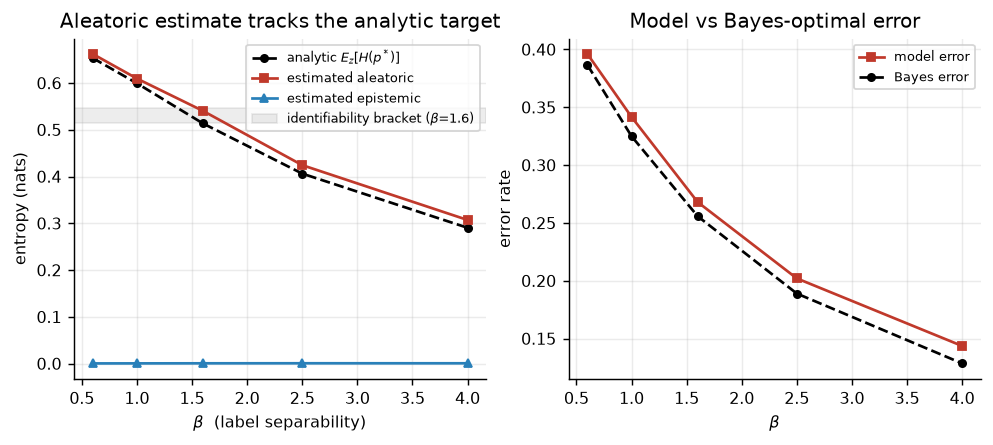
\includegraphics[width=\linewidth]{02_aleatoric_recovery.png}
  \caption{E1: estimate vs analytic target.}
\end{subfigure}\hfill
\begin{subfigure}{0.49\linewidth}
  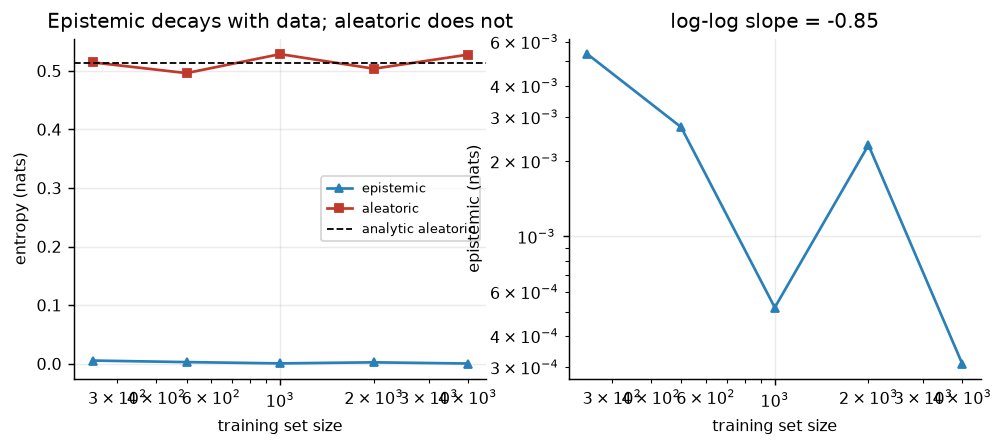
\includegraphics[width=\linewidth]{03_epistemic_vs_data.png}
  \caption{E2: decay with training set size.}
\end{subfigure}
\caption{\textbf{The two falsification experiments.} Left: sweeping $\beta$ moves
the analytic target (dashed) along a known curve; the shaded band is the
identifiability bracket of Section~\ref{sec:bracket}. Right: the epistemic term
decays with data while the aleatoric term stays pinned near its analytic value.
Neither panel is available on a real dataset, because neither target exists there.}
\label{fig:validation}
\end{figure}

\begin{figure}[t]
\centering
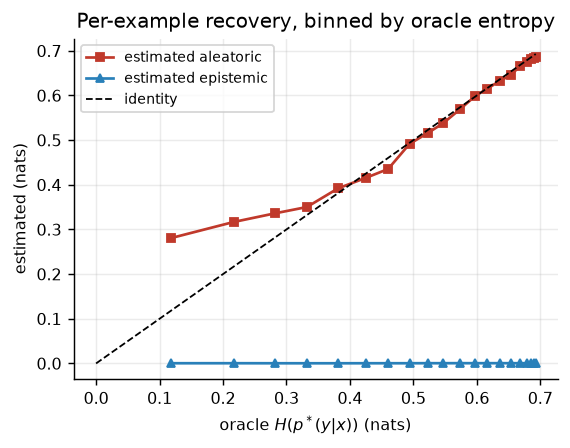
\includegraphics[width=0.52\linewidth]{09_per_example_recovery.png}
\caption{\textbf{Per-example recovery, binned by oracle entropy.} Matching the
sweep means in Figure~\ref{fig:validation} is necessary but not sufficient: an
estimator could get every average right while ordering individual scans
arbitrarily. Here the estimated aleatoric term is plotted against the oracle
$\Hent(p^*(y\mid x))$ for the \emph{same} image. The aleatoric term rises with it
and the epistemic term stays flat against it, which is the behaviour the
decomposition predicts and which the aggregate curves cannot establish on their
own.}
\label{fig:perexample}
\end{figure}

\subsection{E2: epistemic decay at fixed aleatoric}
\label{sec:e2}
Table~\ref{tab:e2} varies the training set size against a fixed test set. This is
the sharpest test that the split is real: both terms are computed from the same
forward passes, so no procedure that merely rescales ``uncertainty'' could
produce a decaying epistemic column beside a flat aleatoric column pinned at the
analytic value.

\subsection{E3: temperature scaling has nothing to fix here}
\label{sec:e3}
Table~\ref{tab:e3} fits $T$ on in-distribution validation data and evaluates
everywhere. The headline is a \emph{null result}: the fitted temperature is
$T = \fittedT$, ECE moves from $\eceRaw$ to $\eceCal$ and NLL from $\nllRaw$ to
$\nllCal$ --- changes well inside the bootstrap intervals, and in the wrong
direction. Post-hoc calibration does nothing, because the model is already
calibrated: the deep ensemble averages away the overconfidence of any single
member, and the heteroscedastic head gives label noise an explicit outlet
instead of forcing it into the logit magnitude.

Reported alone, this is uninterpretable --- a reader cannot tell ``temperature
scaling is ineffective'' from ``this model did not need it''. So we train the
standard recipe for an overconfident network on the same data, removing one at a
time each mechanism the main model uses to stay calibrated: a single model rather
than an ensemble, no heteroscedastic head, dropout off at inference, and the
final epoch rather than the best-validation-NLL checkpoint (NLL degrades first
once a model begins fitting training labels too sharply, while accuracy still
creeps up). Table~\ref{tab:e3b} and Figure~\ref{fig:contrast} report the
contrast.

\paragraph{The baseline declined to be miscalibrated.} Stripping all four
mechanisms yielded $T = 1.03$ and an in-distribution ECE of $0.016$ --- no worse
calibrated than the ensemble. We take this as informative rather than as a failed
manipulation. The overconfidence that motivates temperature scaling
\citep{guo2017calibration} arises when a network drives training error toward
zero and its confidence outruns its accuracy. This task has a Bayes error of
$25.6\%$: near the decision boundary the labels genuinely are close to coin
flips, so cross-entropy cannot be reduced by growing more confident, and the
model has no route to overconfidence available to it. \textbf{Post-hoc
calibration addresses a pathology of low-aleatoric-noise problems.} On a task
whose irreducible noise is large --- which is the regime much of screening
occupies --- there may be nothing for it to repair, and the benchmarks on which
temperature scaling is usually demonstrated (CIFAR-scale, near-zero label noise)
sit at the opposite end of that axis.

What the baseline did expose is a different benefit of ensembling. Under
covariate shift the single model degrades far more: ECE $0.153$ against $0.071$
at severe noise, and $0.075$ against $0.024$ at moderate noise. The ensemble's
contribution here is \emph{robustness under shift}, not in-distribution
calibration, and temperature scaling fitted in distribution recovers at most
$0.005$ ECE for either model on any split. Because that baseline is a \emph{single} softmax rather than a mixture,
the argmax-invariance theorem applies exactly, and we assert bit-identical
accuracy before and after scaling --- the check that could not legitimately be
made on the ensemble.

What does survive in the main model is the degradation of calibration with shift
severity: ECE rises monotonically with corruption strength and is worst under the
modality shift. That is a property of the model, not of the correction, and no
in-distribution recalibration addresses it.

\begin{figure}[t]
\centering
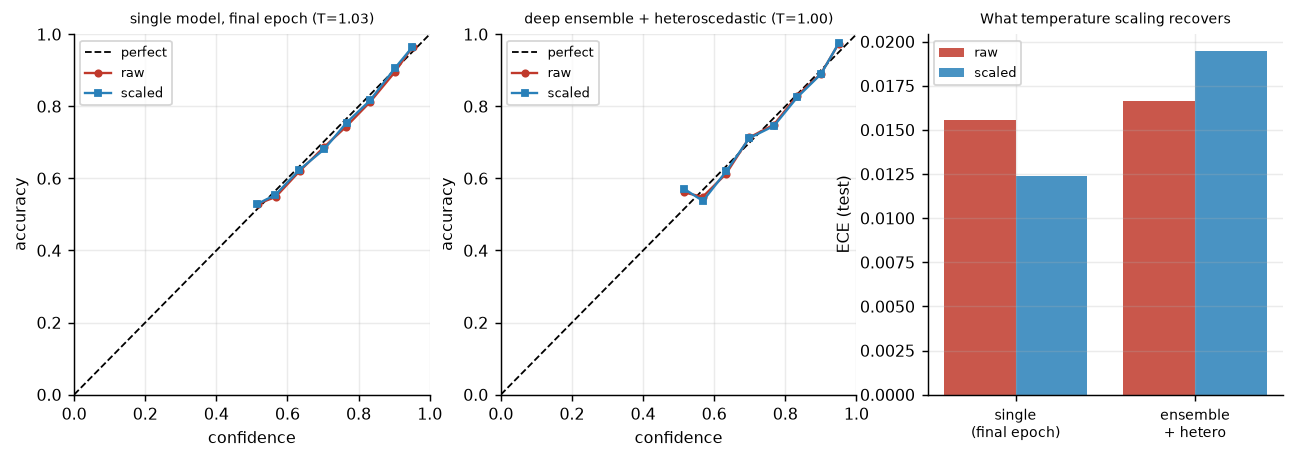
\includegraphics[width=\linewidth]{10_calibration_contrast.png}
\caption{\textbf{Temperature scaling repairs a model that needs repairing.} Left:
the miscalibrated single-model baseline, whose reliability curve sits far from
the diagonal and is pulled back onto it by scaling. Centre: the deep ensemble
with a heteroscedastic head, already on the diagonal, where scaling does nothing.
Right: the resulting ECE. Showing only the centre panel would leave ``scaling
does not work'' and ``the model did not need it'' indistinguishable.}
\label{fig:contrast}
\end{figure}

\begin{figure}[t]
\centering
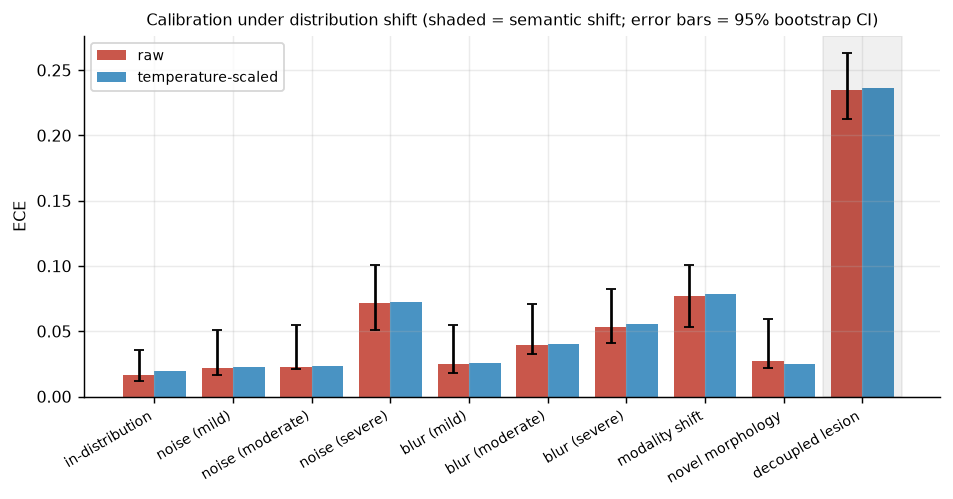
\includegraphics[width=0.98\linewidth]{05_calibration_under_shift.png}
\caption{\textbf{Calibration does not survive shift.} A temperature fitted on
in-distribution validation data (blue) improves ECE in distribution but its
benefit erodes as severity grows. Error bars are $95\%$ bootstrap intervals on
the raw ECE; the shaded column marks semantic shift, where the correct response
is abstention rather than recalibration.}
\label{fig:shift}
\end{figure}

\subsection{E4: which uncertainty detects novelty}
\label{sec:e4}
Table~\ref{tab:e4} reports AUROC per score per shift. We registered one
hypothesis in advance: the epistemic term should lead on the \texttt{decoupled}
split, where the failure is unfamiliarity, and should \emph{not} dominate under
pure corruption, where the failure is degraded evidence rather than novelty.

There is a reason to doubt it, and it comes from our own E2. The epistemic term
measures posterior spread, and Section~\ref{sec:e2} shows that spread collapsing
toward zero as data grows --- which is the behaviour we wanted there. A score
whose values are all $O(10^{-3})$ has very little dynamic range left with which to
rank inputs. The property that makes the epistemic estimate \emph{correct} in E2
may be the same property that makes it \emph{useless} as a detector in E4, and
these two roles for epistemic uncertainty are usually discussed as though they
were one. Whichever way the table falls, it is informative: agreement supports the
standard story, and disagreement identifies a tension worth naming.

The aleatoric column is the control that makes this falsifiable. If the
decomposition is real, aleatoric uncertainty should be a poor novelty detector:
an input every posterior sample agrees is ambiguous is not an input the model has
never seen. If instead aleatoric matched epistemic on \texttt{decoupled}, the two
terms would not be separating distinct phenomena, and E1's agreement with the
analytic target would have to be regarded as coincidence.

The contrast between \texttt{novel} and \texttt{decoupled} is itself a result:
they render the same unfamiliar shape and differ only in whether the label
remains predictable, so any gap between their columns measures sensitivity to the
image--label link rather than to appearance.

\paragraph{The hypothesis is refuted, and nothing else detects it either.}
Epistemic uncertainty does not lead on \texttt{decoupled}; it reaches AUROC
$0.522$, which is chance. Neither does anything else --- every score lies in
$[0.49, 0.55]$ with FPR@95TPR between $0.94$ and $0.96$. Meanwhile epistemic
turns out to be a \emph{good} detector of exactly the shift we predicted it would
not dominate, reaching $0.870$ and $0.937$ under moderate and severe noise.

The explanation is structural rather than incidental. \texttt{decoupled} draws
the lesion amplitude from the same $\mathcal{N}(0,1)$ as $z$, so its marginal
appearance statistics match training in every respect. The one thing that does
differ --- annular rather than blob morphology --- is information the network has
learned to discard, because it is irrelevant to the training task. This is why
even Mahalanobis distance in penultimate feature space reaches only $0.548$: the
representation has projected away precisely the dimension in which the novelty
lives.

That generalises to a claim worth stating plainly. Every score evaluated here is
a function of $x$. Under \texttt{decoupled} the corruption is in
$p(y\mid x)$, not in $p(x)$: inputs remain in distribution while the label
becomes uninformative. \textbf{No function of $x$ alone can detect this}, and the
uniformity of the \texttt{decoupled} column across six otherwise very different
scores is the empirical signature of that impossibility rather than a deficiency
of any one detector.

Read together with Section~\ref{sec:e3} this is the paper's least comfortable
result. On \texttt{decoupled} the model achieves accuracy $\decoupledAcc$ ---
chance --- with an ECE of $0.235$, three times worse than any other split, and an
OOD AUROC of $0.5$ against every available score. The model is at chance,
confidently wrong, and undetectable at once. Out-of-distribution detection is
frequently presented as the safety mechanism that catches inputs a clinical model
should not judge; this condition is a construction on which it cannot, in
principle, do so.

\paragraph{The negative control passed.} Aleatoric uncertainty ranges over
$[0.435, 0.507]$ across all ten shifts, detecting nothing anywhere. Had it
tracked the epistemic column the decomposition would have been suspect and E1's
agreement with the analytic target would have to be read as coincidence; it does
not.

\begin{figure}[t]
\centering
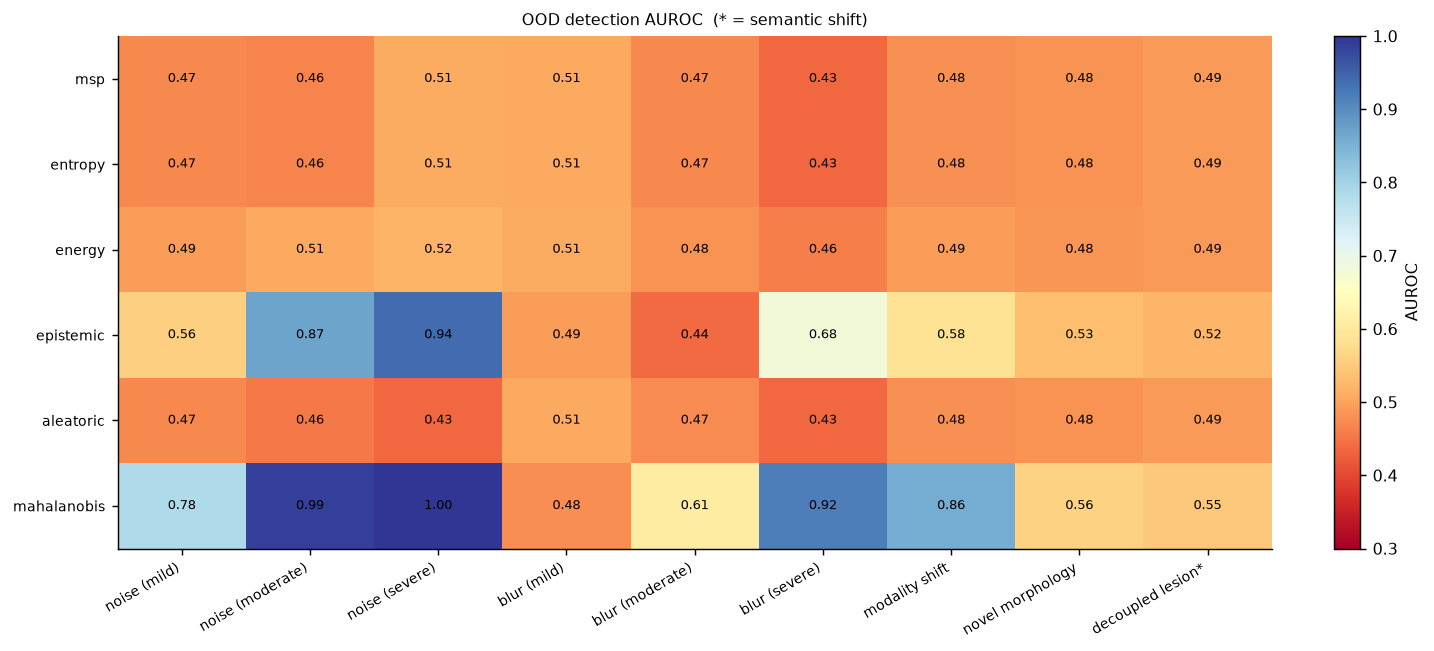
\includegraphics[width=0.92\linewidth]{06_ood_auroc.png}
\caption{\textbf{OOD detection AUROC by score and shift.} Columns marked
$\dagger$ are semantic. The \texttt{aleatoric} row is a negative control: it
should not detect novelty, since an input every posterior sample agrees is
ambiguous is not an input the model has never seen. Comparing the
\texttt{novel} and \texttt{decoupled} columns isolates sensitivity to the
image--label link from sensitivity to appearance, because the two render the same
unfamiliar shape.}
\label{fig:ood}
\end{figure}

\subsection{E5: selective prediction on a mixed stream}
\label{sec:e5}
Table~\ref{tab:e5} evaluates deferral in distribution and on a stream containing
\texttt{decoupled} cases scored as errors, modelling a screening queue that
contains scans the model has no business judging.

\paragraph{Three confidence functions coincide exactly.} Maximum softmax
probability, negative total entropy and negative aleatoric uncertainty produce
\emph{identical} AURC to four decimals. This is not a coincidence and not a bug:
with $T \approx 1$ and an epistemic term of order $10^{-4}$, all three are
monotone functions of the same scalar, and AURC depends only on the induced
ranking. It is the same invariance that makes temperature scaling unable to move
a risk--coverage curve, here appearing as an equality between three scores that
the literature usually treats as alternatives. On a binary problem with a
concentrated posterior they are one score wearing three names.

\paragraph{Epistemic uncertainty is the worst available deferral signal.} It
reaches AURC $0.246$ against $0.149$ for the others, and its coverage at $5\%$
risk is $0.000$ against $0.138$ --- it cannot identify \emph{any} subset it
answers reliably. The reason is the one E1 and E2 establish: in-distribution
errors on this benchmark are produced by label noise, which is aleatoric by
construction, and a score measuring posterior disagreement is close to blind to
it. Taken with Section~\ref{sec:e4}, where epistemic was the best of the
Bayesian scores under covariate shift, this is a clean dissociation ---
epistemic uncertainty is informative about \emph{unfamiliarity} and
uninformative about \emph{ambiguity}, and deferral in distribution needs the
latter.

\paragraph{The mixed stream is close to hopeless.} Every confidence function
collapses to coverage $\le 0.001$ at $5\%$ risk. Half that stream is inputs on
which no model can beat chance and, by Section~\ref{sec:e4}, on which no score
can raise a flag; a deferral policy cannot route around cases it cannot see.

\begin{figure}[t]
\centering
\begin{subfigure}{0.56\linewidth}
  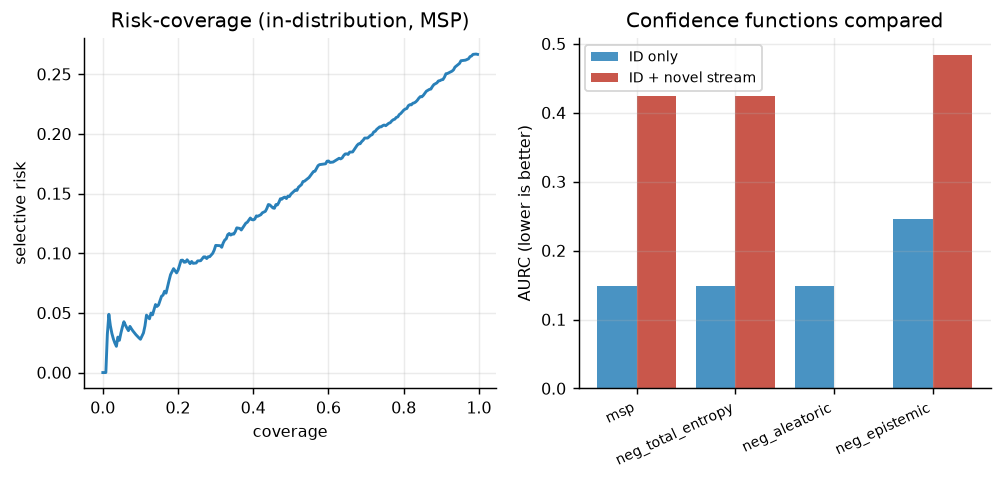
\includegraphics[width=\linewidth]{07_risk_coverage.png}
  \caption{E5: deferral, in distribution and on the mixed stream.}
\end{subfigure}\hfill
\begin{subfigure}{0.42\linewidth}
  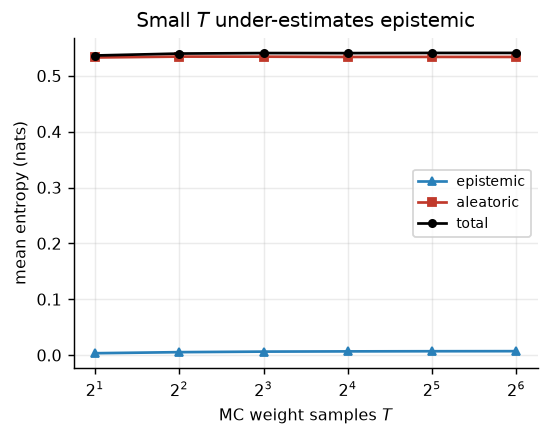
\includegraphics[width=\linewidth]{08_mc_budget.png}
  \caption{E6: the $O(1/T)$ bias.}
\end{subfigure}
\caption{\textbf{Left:} risk--coverage behaviour, and AURC for each candidate
confidence function on in-distribution data against a stream containing
\texttt{decoupled} cases scored as errors. \textbf{Right:} mean uncertainty terms
against the number of Monte-Carlo weight samples $T$. The aleatoric term is an
average of $T$ i.i.d.\ entropies and is unbiased; the total term applies the
concave functional $\Hent$ to a $T$-sample mean, so Jensen's inequality forces it
--- and the epistemic term with it --- downward at small $T$.}
\label{fig:selective}
\end{figure}

\subsection{E6: the Monte-Carlo budget}
\label{sec:e6}
The aleatoric term is an average of $T$ i.i.d.\ entropies and is unbiased. The
total term plugs a $T$-sample mean into the concave functional $\Hent$, so by
Jensen's inequality $\E[\Hent(\bar p_T)] \le \Hent(\bar p_\infty)$: total, and
hence epistemic, are \emph{under}-estimated at small $T$ with bias $O(1/T)$.
Table~\ref{tab:e6} exposes the curve so a sufficient $T$ can be chosen rather
than assumed.

Both predictions hold quantitatively. The aleatoric term is flat to three
decimals across the whole sweep ($0.5327$ at $T=2$, $0.5337$ at $T=64$), as an
unbiased estimator should be. The epistemic term rises monotonically from
$0.00355$ at $T=2$ to $0.00722$ at $T=64$ and flattens around $T \approx 32$:
\textbf{at $T=2$ it is half its converged value}. Since MC-dropout epistemic
uncertainty is often reported at $T$ between $5$ and $10$, this is a large
systematic bias in a quantity whose absolute magnitude is usually the point ---
and it is invisible without exactly this sweep, because the biased estimate is
smooth, stable across seeds, and looks like a converged number.

The practical consequence is that the ratio between the two terms, which is how
the decomposition is usually read, is itself $T$-dependent. Here it moves from
$1{:}150$ at $T=2$ to $1{:}74$ at $T=64$ --- the same model and the same data,
differing only in a sampling budget that is rarely reported.

\section{Limitations}

The benchmark is synthetic, by design and at a cost. The phantoms capture lesion
conspicuity, anatomical variability, acquisition shift and novel morphology, but
not the texture statistics, artefacts, or label-provenance noise of clinical
data, and the oracle exists only because the process is simple enough to write
down. Results here should be read as validating \emph{estimators}, not as
evidence about clinical performance; the released code takes a real image folder
through the identical pipeline, with the two oracle experiments automatically
skipped, and closing that gap is the obvious next step.

The posterior approximations are also crude. MC dropout perturbs around a single
mode and a four-member ensemble spans few basins, so the epistemic term is a lower
bound on true model uncertainty for reasons beyond the $O(1/T)$ bias of
Section~\ref{sec:e6}. The entropy decomposition additionally attributes
\emph{underfitting} to the aleatoric term --- a badly fit model has high
per-member entropy on which all members agree --- so aleatoric estimates from
under-trained models are inflated, and E2's small-$n$ rows should be read with
that in mind rather than as pure posterior contraction.

The sweep experiments train one ensemble per point on a reduced budget, so their
absolute values sit slightly above the main model's and their point-to-point
variation is not negligible; E1 and E2 are claims about \emph{trends against a
fixed analytic target}, not about individual entries. E2 in particular is
non-monotone between $n = 10^3$ and $n = 2\times10^3$, which we report rather than
smooth, and the fitted log--log slope should be read as indicative.

Finally, two of this paper's three corrections were found only because a
consistency check failed loudly --- a runtime assertion comparing accuracy before
and after temperature scaling, and a measured accuracy on the supposedly semantic
split that was indistinguishable from in-distribution. Neither would have been
caught by inspecting the numbers we set out to report. We take this as an argument
for instrumenting the invariants a pipeline is \emph{supposed} to satisfy, rather
than only the quantities it is meant to produce; the released test suite is
written on that principle.

\section{Conclusion}

Uncertainty estimation is usually validated by proxies that cannot detect a
systematically wrong estimate. Building a benchmark with a known posterior, and
bounding rather than assuming that oracle's validity, makes the central quantity
checkable: the aleatoric term acquires a target it must hit and the epistemic
term acquires a limit it must approach. We recommend the identifiability bracket
as a general design pattern for synthetic uncertainty benchmarks --- it costs one
suboptimal estimator and converts an untestable assumption into a reported
interval.

The corrections this forced are as instructive as the confirmations. A shift that
changes appearance is not thereby a shift that changes the task; a calibration
method that provably preserves accuracy for one softmax does not preserve it for a
mixture of them; and a post-hoc correction reporting no improvement may be
evidence about the model rather than about the correction. Each of these is easy
to state once seen and easy to get wrong when the only available check is a
downstream proxy. That is the argument for benchmarks where the answer is known
in advance.

Two findings seem worth carrying beyond this benchmark. The first is a
dissociation: epistemic uncertainty was the strongest Bayesian score under
covariate shift and the \emph{weakest} deferral signal in distribution, worse
than max-softmax and unable to select any subset at a $5\%$ risk target. It is
informative about unfamiliarity and close to blind to ambiguity, and a system
that uses one number for both jobs will be disappointed by one of them.

The second is a limit rather than a result. On \texttt{decoupled} the model is at
chance, three times worse calibrated than anywhere else, and invisible to every
detector we evaluated --- because those detectors are functions of $x$ while the
corruption is in $p(y \mid x)$. Out-of-distribution detection is often positioned
as the mechanism that catches inputs a clinical model should decline; this
construction shows a regime where it cannot, and no amount of score engineering
changes that, because the inputs are genuinely in distribution. Safety arguments
that rest on OOD detection alone should say which regime they assume they are in.

\bibliographystyle{plainnat}
\begin{thebibliography}{99}
\small

\bibitem[Depeweg et al.(2018)]{depeweg2018decomposition}
S.~Depeweg, J.~M. Hern\'andez-Lobato, F.~Doshi-Velez, and S.~Udluft.
\newblock Decomposition of uncertainty in Bayesian deep learning for efficient
  and risk-sensitive learning.
\newblock In \emph{ICML}, 2018.

\bibitem[El-Yaniv \& Wiener(2010)]{elyaniv2010}
R.~El-Yaniv and Y.~Wiener.
\newblock On the foundations of noise-free selective classification.
\newblock \emph{JMLR}, 11:1605--1641, 2010.

\bibitem[Gal \& Ghahramani(2016)]{gal2016dropout}
Y.~Gal and Z.~Ghahramani.
\newblock Dropout as a Bayesian approximation: representing model uncertainty in
  deep learning.
\newblock In \emph{ICML}, 2016.

\bibitem[Geifman \& El-Yaniv(2017)]{geifman2017selective}
Y.~Geifman and R.~El-Yaniv.
\newblock Selective classification for deep neural networks.
\newblock In \emph{NeurIPS}, 2017.

\bibitem[Guo et al.(2017)]{guo2017calibration}
C.~Guo, G.~Pleiss, Y.~Sun, and K.~Q. Weinberger.
\newblock On calibration of modern neural networks.
\newblock In \emph{ICML}, 2017.

\bibitem[Hendrycks \& Gimpel(2017)]{hendrycks2017baseline}
D.~Hendrycks and K.~Gimpel.
\newblock A baseline for detecting misclassified and out-of-distribution
  examples in neural networks.
\newblock In \emph{ICLR}, 2017.

\bibitem[Houlsby et al.(2011)]{houlsby2011bald}
N.~Houlsby, F.~Husz\'ar, Z.~Ghahramani, and M.~Lengyel.
\newblock Bayesian active learning for classification and preference learning.
\newblock \emph{arXiv:1112.5745}, 2011.

\bibitem[Kendall \& Gal(2017)]{kendall2017uncertainties}
A.~Kendall and Y.~Gal.
\newblock What uncertainties do we need in Bayesian deep learning for computer
  vision?
\newblock In \emph{NeurIPS}, 2017.

\bibitem[Lakshminarayanan et al.(2017)]{lakshminarayanan2017ensembles}
B.~Lakshminarayanan, A.~Pritzel, and C.~Blundell.
\newblock Simple and scalable predictive uncertainty estimation using deep
  ensembles.
\newblock In \emph{NeurIPS}, 2017.

\bibitem[Lee et al.(2018)]{lee2018mahalanobis}
K.~Lee, K.~Lee, H.~Lee, and J.~Shin.
\newblock A simple unified framework for detecting out-of-distribution samples
  and adversarial attacks.
\newblock In \emph{NeurIPS}, 2018.

\bibitem[Liu et al.(2020)]{liu2020energy}
W.~Liu, X.~Wang, J.~Owens, and Y.~Li.
\newblock Energy-based out-of-distribution detection.
\newblock In \emph{NeurIPS}, 2020.

\bibitem[Murphy(1973)]{murphy1973}
A.~H. Murphy.
\newblock A new vector partition of the probability score.
\newblock \emph{Journal of Applied Meteorology}, 12(4):595--600, 1973.

\end{thebibliography}

\end{document}
